\section{Particle Identification}\label{section:star_PIDdEdx}
Specific ionization energy loss, the $dE/dx$, is a function of the~magnitude of a~particle momentum.  In this section the particle identification with help of $dE/dx$  is described.
Due to a~low particle multiplicity and lack of signal in VPDs on the outgoing proton side (presence of the rapidity gap) in SD events, the time of collision is not defined precisely enough, therefore, the particle identification  by the TOF is not possible
and the~analysis was limited to identification only by $dE/dx$. 

The ionization energy loss of charged particles in material
is given by the Bethe-Bloch formula and for
the STAR \ac{TPC} by the more precise Bichsel formula~\cite{Bichsel:2006cs}.
The particle type can be determined by comparison of particle's $dE/dx$ with the Bethe-Bloch (Bichsel) expectations.
Figure \ref{fig:star_dedx} shows the  $dE/dx$ versus rigidity $q\times p$ for particles in $|\eta| < 0.7$. Particles are  well separated at low $|q\times p|$, whereas at higher $|q\times p|$ the $dE/dx$ of different particle species starts to
overlap: $e^\pm$ and $K^\pm$ merge at $\sim0.4$~GeV/c, $K^\pm$ and
$\pi^\pm$ merge at $\sim0.65$~GeV/c, and $p(\bar{p})$ and $\pi^\pm$ merge
at $\sim1$~GeV/c. 
\begin{figure}[b!]
	\centering
	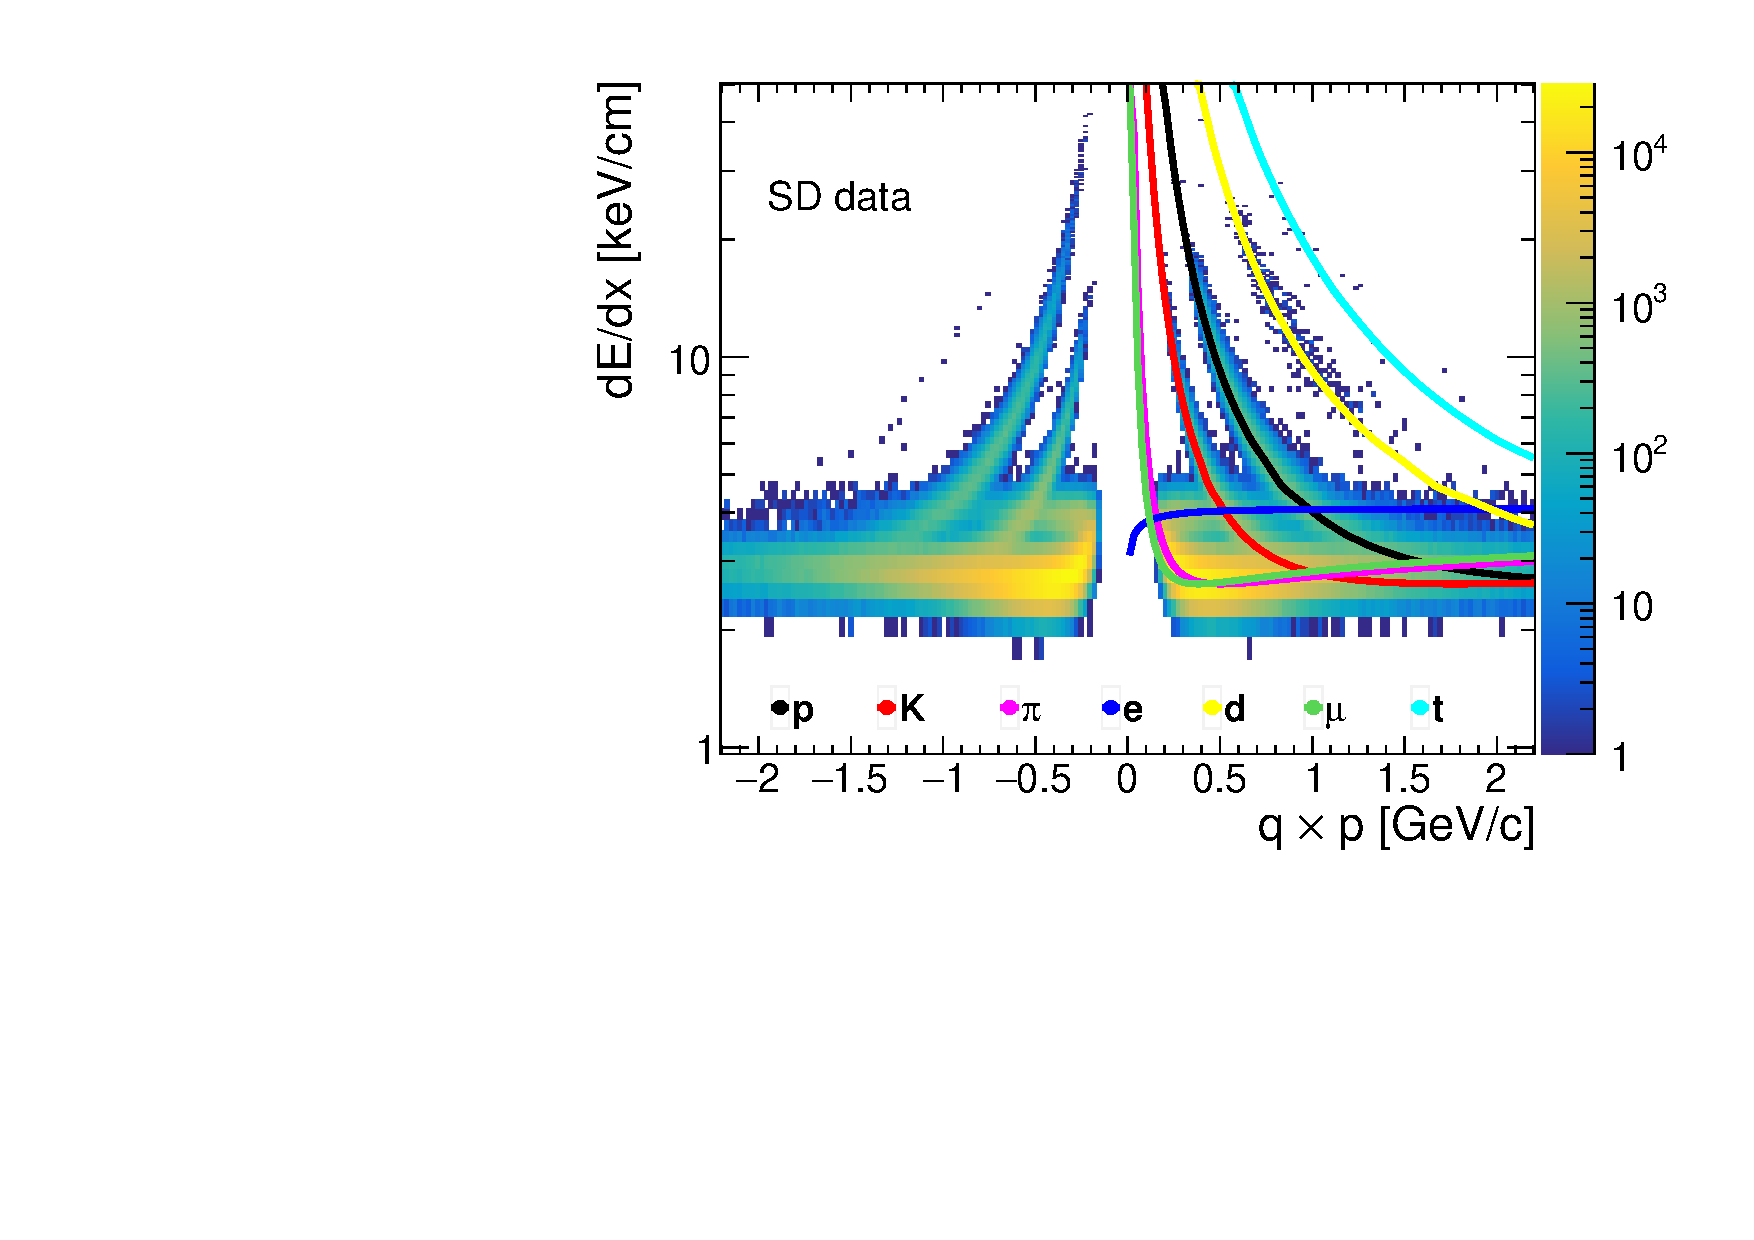
\includegraphics[width=0.65\linewidth, page=1]{chapters/chrgSTAR/img/dEdx/SDT_dEdx.pdf}
	\caption[Specific ionization
	energy loss $dE/dx$ as a function of rigidity $q\times p$ for particles
	in $|\eta| < 0.7$]{Specific ionization
		energy loss $dE/dx$ as a function of rigidity $q\times p$ for particles
		in $|\eta| < 0.7$. The Bichsel predictions for each particle species are also shown.}
	\label{fig:star_dedx}
\end{figure} 
%\FloatBarrier
\noindent Since the $dE/dx$ distribution for a given particle type
is not Gaussian, the following variable for each particle type was defined:
\begin{equation}
n\sigma^i_{dE/dx}=\ln\left(\frac{dE/dx}{(dE/dx)_i^\textrm{{BB}}}\right)/\sigma
\label{eq:nsigma}
\end{equation}
where $(dE/dx)_i^\textrm{{BB}}$ is the Bethe-Bloch (Bichsel) expectation
of $dE/dx$ for the given particle type $i$ $(i =
\pi, K, p)$, $\sigma$ - the~relative $dE/dx$ resolution.
The expected value of $n\sigma^i_{dE/dx}$ for the~particle under consideration is  $0$  and the width equals to $1$. The sample $n\sigma^i_{dE/dx}$ distribution for $\pi^{\pm}$, $K^\pm$ and $p(\bar{p})$ in one $\xi$ range, $0.02 < \xi < 0.05$, is shown  in Fig.~\ref{fig:dEdx_nsigma}.
\begin{figure}[h!]
	
	\centering
	\begin{subfigure}{.49\textwidth}
		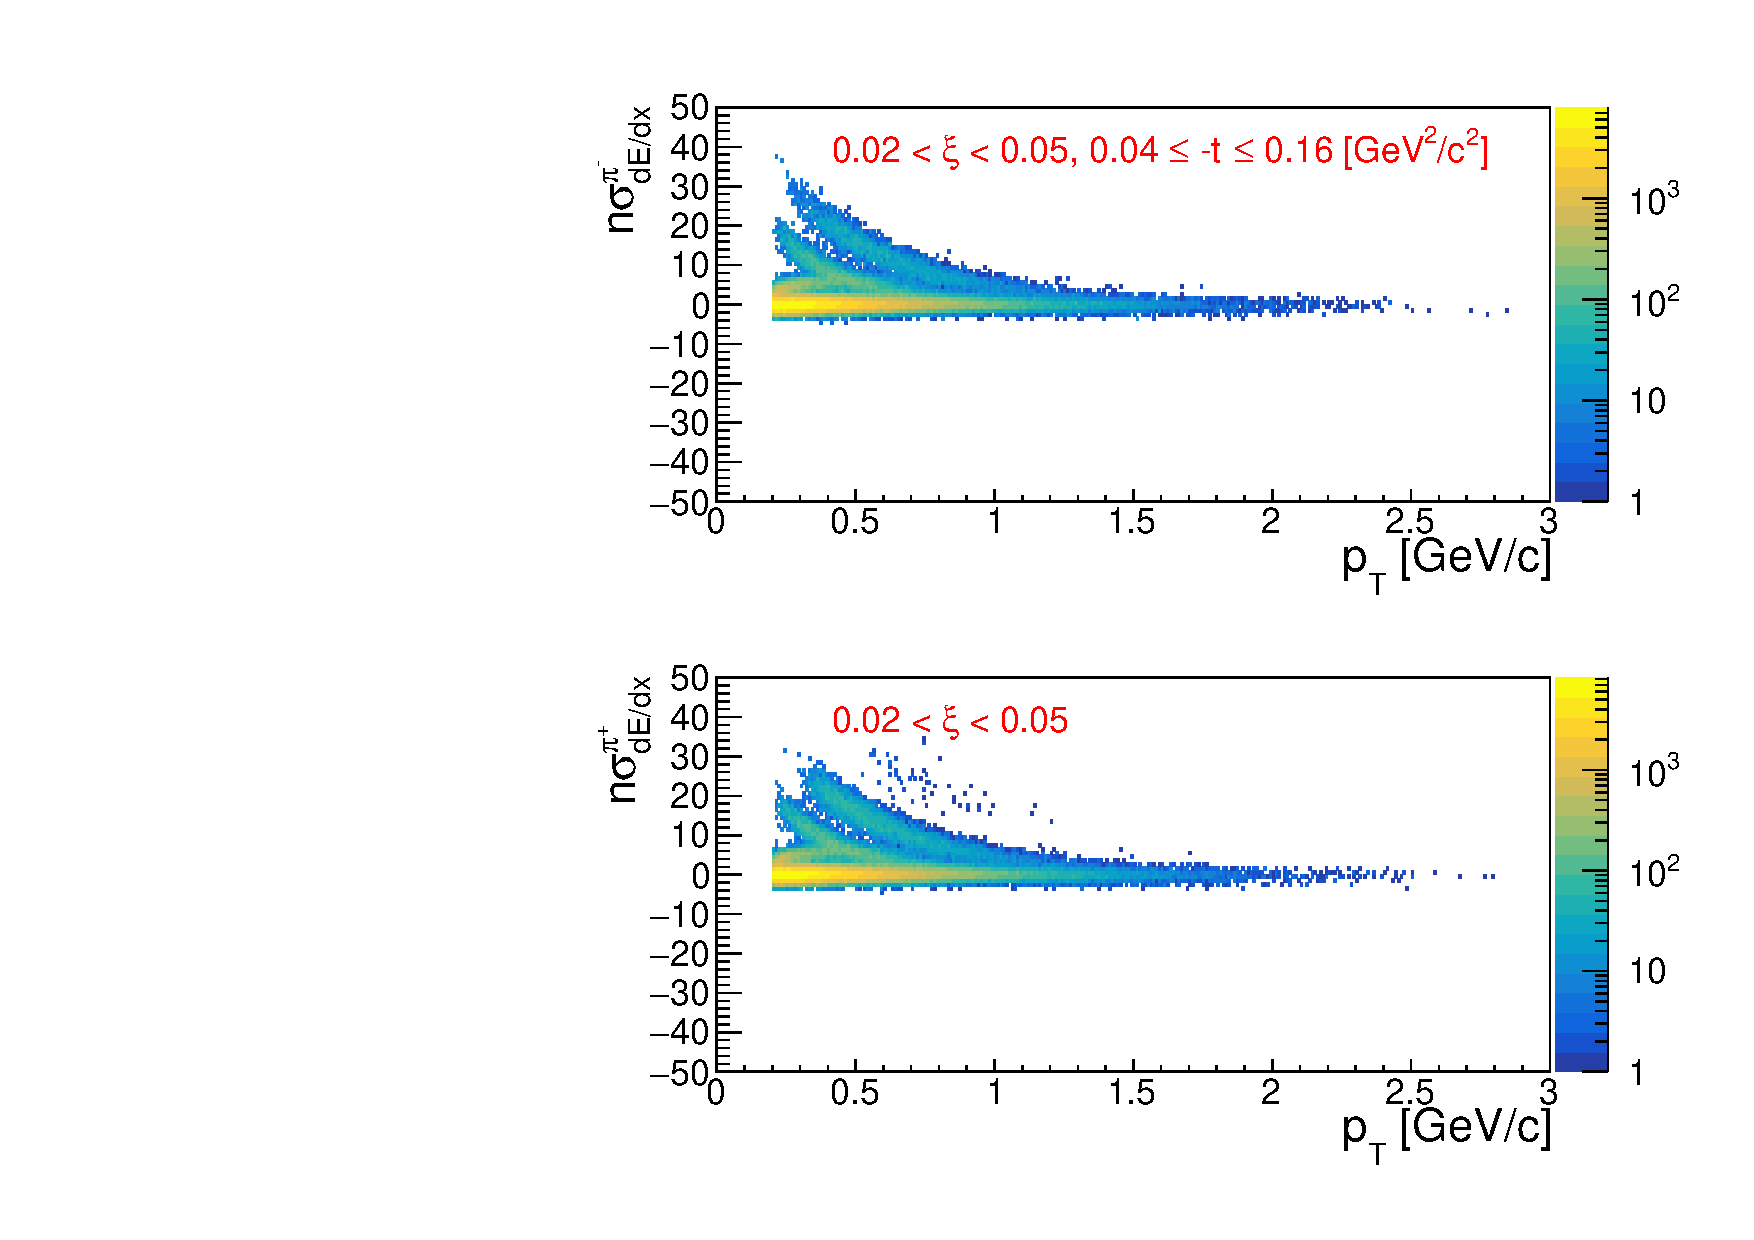
\includegraphics[width=\linewidth, page=1]{chapters/chrgSTAR/img/dEdx/fit2019_2dNsigma_0_0.pdf}
	\end{subfigure}
	\begin{subfigure}{.49\textwidth}
		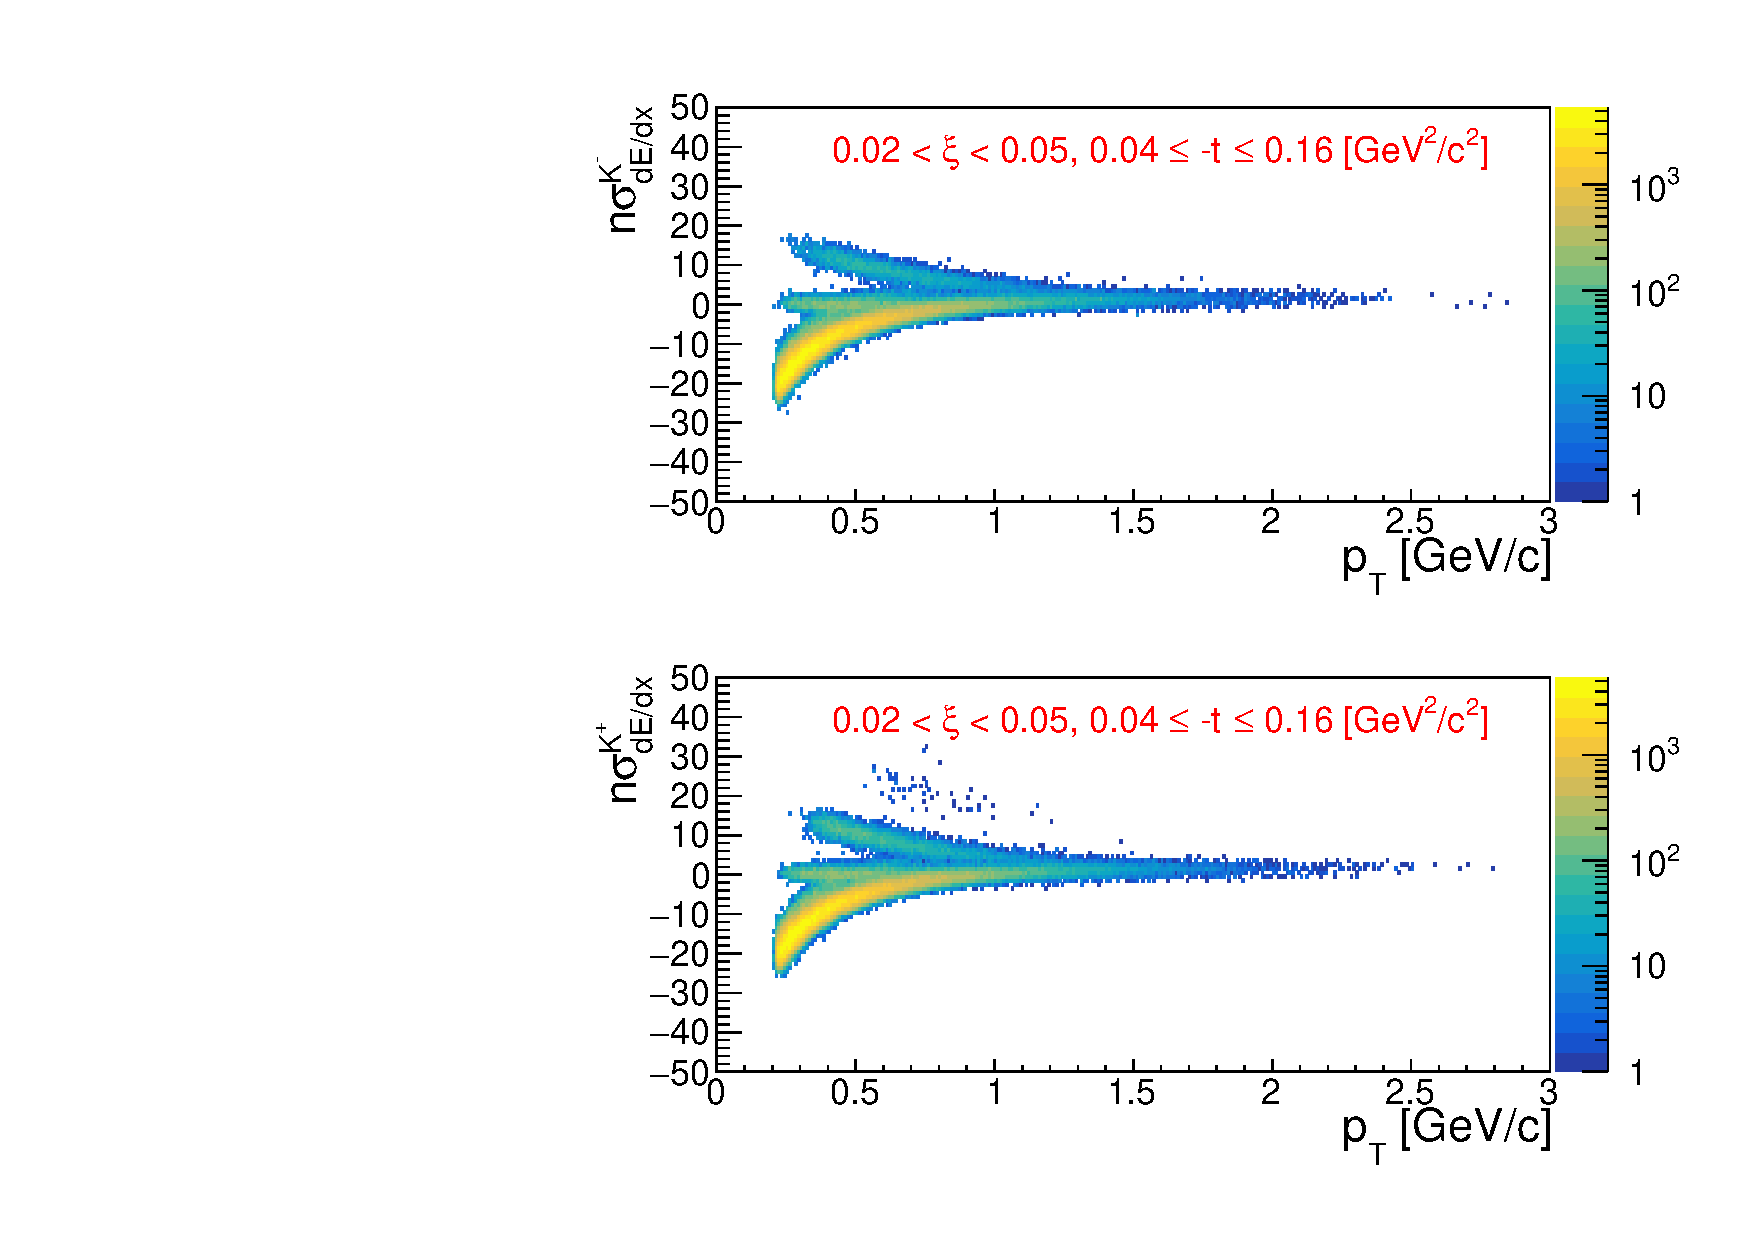
\includegraphics[width=\linewidth, page=1]{chapters/chrgSTAR/img/dEdx/fit2019_2dNsigma_0_1.pdf}
	\end{subfigure}
	\begin{subfigure}{.49\textwidth}
		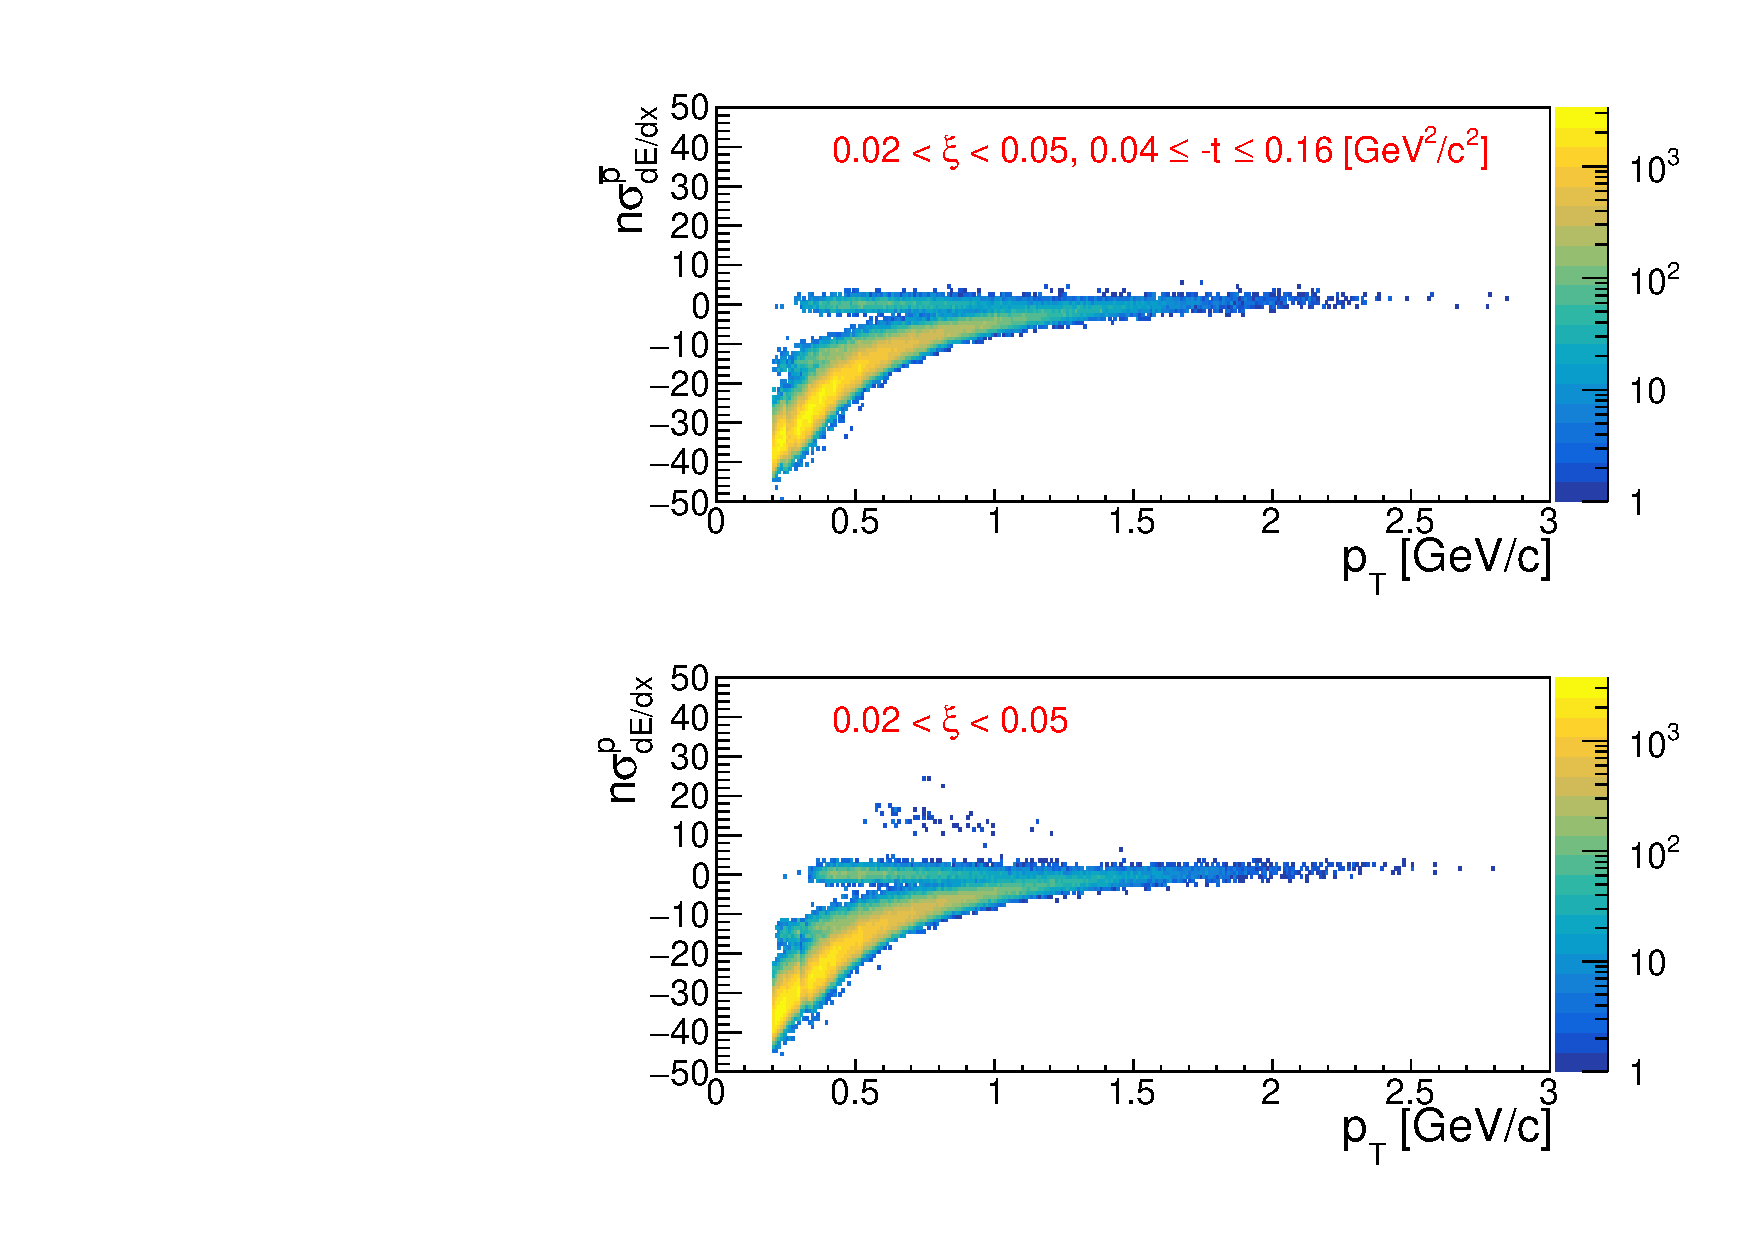
\includegraphics[width=\linewidth, page=1]{chapters/chrgSTAR/img/dEdx/fit2019_2dNsigma_0_2.pdf}
	\end{subfigure}
	\begin{minipage}{.49\textwidth}
			\caption{
			The $n\sigma^{i}_{dE/dx}$ variable for particle $i^\pm$ versus $p_\textrm{T}$. Particles are restricted in $|\eta| < 0.7$ and corrected for the energy loss (mass of $i^\pm$-particle was taken)~\cite{supplementaryNote} and vertexing.}
		\label{fig:dEdx_nsigma}
	\end{minipage}
	\vspace{1em}
\end{figure}

\begin{figure}[h!]
	\centering
	\begin{subfigure}{.49\textwidth}
		\includegraphics[width=\linewidth, page=9]{chapters/chrgSTAR/img/dEdx/fit2019_secondStep_0_0.pdf}
	\end{subfigure}
	\begin{subfigure}{.49\textwidth}
		\includegraphics[width=\linewidth, page=7]{chapters/chrgSTAR/img/dEdx/fit2019_thirdStep_1_0.pdf}
	\end{subfigure}\par
	\begin{subfigure}{.49\textwidth}
		\includegraphics[width=\linewidth, page=5]{chapters/chrgSTAR/img/dEdx/fit2019_thirdStep_2_0.pdf}
	\end{subfigure}
	\begin{minipage}{.49\textwidth}
		\caption{Distributions of (top left) $n\sigma^{\pi^\pm}_{dE/dx}$ for $\pi^\pm$, (top right) $n\sigma^{K^\pm}_{dE/dx}$ for $K^\pm$ and (bottom left) $n\sigma^{\bar{p}/p}_{dE/dx}$ for $\bar{p}/p$ in sample  $p_\textrm{T}$ bin and sample $\xi$ range  shown for each particle species. Particles are corrected for  energy loss~\cite{supplementaryNote} and vertexing. The curves represent the Gaussian fits to the $n\sigma^{i}_{dE/dx}$ distributions.}
		\label{fig:dEdx_fit_example}
	\end{minipage}
	
\end{figure}


\noindent Figure \ref{fig:dEdx_fit_example}
shows the $n\sigma^{\pi^\pm}_{dE/dx}$,$n\sigma^{K^\pm}_{dE/dx}$ and $n\sigma^{p(\bar{p})}_{dE/dx}$ distributions for  $0.6 < p_\textrm{T} < 0.65$~GeV/c  in the~$\xi$ range, $0.02 < \xi < 0.05$, each corrected for the energy loss (mass of $i$-particle was assumed)~\cite{supplementaryNote} and vertexing  (other $p_\textrm{T}$ bins are shown in Appendix~\ref{appendix:dEdxFits}). To extract the  particle yield for a given particle type,
a~multi-Gaussian fit is applied to the $n\sigma^i_{dE/dx}$ distribution in each $p_\textrm{T}$ bin and $\xi$ range. The parameters of the multi-Gaussian fit are the centroids $\mu_{i^-/i^+}$, widths $\sigma_{i^-/i^+}$, sums  and ratios  of yields $C_{i^-/i^+}$, $r_{i^-/i^+}$ for negative $i^-$ and positive $i^+$ particles ($\pi^\pm$, $e^\pm$, $K^\pm$, $p$ and $\bar{p}$). The~positive and negative particle
$n\sigma^{i}_{dE/dx}$-distributions are fitted simultaneously, where the~centroids and widths are kept the same for particle
and antiparticle. 
In some $p_\textrm{T}$ regions, the~fit does not converge,
because different particle species are not well separated  there. Therefore, multiple steps of the~fitting procedure  are performed to reduce the number of free parameters in the final fit and ensure its stability. Almost all centroids and widths are constrained  by a~function with free parameters $p_k$, where $k \in \mathbb N$.  The function is chosen to describe the data as best as possible.
Since $dE/dx$ is a~function of the~particle's momentum and its shape should be independent of the~process under study, the values of $p_k$  are obtained only for events with $0.02 < \xi < 0.05$ and kept the same for other $\xi$ ranges. 
%The electron contributions are  fixed, but separately for each $\xi$ range. 
The~electron parameters are limited based on the difference between data and MC. Their contributions are fitted only in the~first analysed $p_\textrm{T}$ range, separately for each particle species and $\xi$ range. For higher $p_\text{T}$ ranges, they are estimated from PYTHIA~8 embedding MC, and scaled according to the~ratio of PYTHIA~8 predictions and  contributions fitted in the~first $p_\textrm{T}$ bin.
The procedure slightly differs for different particle types. In each step, the~multi-Gaussian fit is performed first, then the~widths and centroids are fitted  in  $p_\textrm{T}$ ranges in which the fit applied to $n\sigma^{i}_{dE/dx}$ converges. Later,  the~widths and centroids are extrapolated to other $p_\textrm{T}$ ranges, in which particle species are not well separated:
%\newpage
\begin{enumerate}
	\item  $\pi^{\pm}$:
		\begin{itemize}
			\item Step 1 (Fig. ~\ref{fig:dEdx_fit_parametersPi}):
			\begin{itemize}
				\renewcommand\labelitemi{--}
				\item Analyze data with $0.2 < p_\textrm{T} < 0.65$~GeV/c
				\item Fit  $\mu_{\pi^-/\pi^+}$ and $\sigma_{\pi^-/\pi^+}$ as a function of $p_\textrm{T}$ with a polynomial  $p_0p_\textrm{T}^3+p_1p_\textrm{T}^2+p_2p_\textrm{T}+p_3$
				\item Fit $r_{e^-/e^+}$ as a function of $p_\textrm{T}$ with a polynomial $p_0p_\textrm{T}^2+p_1p_\textrm{T}+p_2$
				\item Fit  $C_{e^-/e^+}$, $\mu_{K^-/K^+}$ as a functions of $p_\textrm{T}$ with $p_0\exp\left(p_1p_\textrm{T}\right)+p_2$
				\item Fit  $\mu_{e^-/e^+}$ as a function of $p_\textrm{T}$ with $p_0\exp\left[-\left(p_1p_\textrm{T}\right)^{p_2}\right]$ 
				\item Fit $\sigma_{K^-/K^+}$ as a function of $p_\textrm{T}$, for $0.3<p_\textrm{T}<0.5$~GeV/c, with constant $p_0$ 
				\item Fit  $\mu_{\bar{p}/p}$ and $\sigma_{\bar{p}/p}$ as a function of $p_\textrm{T}$ with $p_0\exp\left(p_1p_\textrm{T}\right)$
			\end{itemize}
			\item Step 2:
				\begin{itemize}
					\renewcommand\labelitemi{--}
					\item $\sigma_{e^-/e^+}$ fixed to $1.2$ and $0.8$ for $0.2<p_\textrm{T}<0.4$ and $0.4<p_\textrm{T}<0.7$, respectively
					\item Fit $\sigma_{K^-/K^+}$ as a function of $p_\textrm{T}$, for $0.3<p_\textrm{T}<0.7$~GeV/c, with constant $p_0$ and fix it to the~value of $p_0$
					\item  The rest parameters from Step 1 are fixed to the~values calculated from functions obtained in Step 1: $\mu_{\pi^-/\pi^+}$, $\sigma_{\pi^-/\pi^+}$, , $r_{e^-/e^+}$, $C_{e^-/e^+}$, $\mu_{e^-/e^+}$ , $\mu_{K^-/K^+}$, $\mu_{\bar{p}/p}$, $\sigma_{\bar{p}/p}$
				\end{itemize}	
		\end{itemize}		
\end{enumerate} 

\begin{enumerate}
	\item[2.] $K^\pm$:
	\begin{itemize}
		\item Step 1 (Fig. ~\ref{fig:dEdx_fit_parametersK}):
		\begin{itemize}
			\renewcommand\labelitemi{--}
			\item Analyze data with $0.2 < p_\textrm{T} < 0.6$~GeV/c
			\item Fit  $\mu_{\pi^-/\pi^+}$  as a function of $p_\textrm{T}$ with $-\exp\left(p_0+p_1p_\textrm{T}\right)$
			\item Fit $\sigma_{\pi^-/\pi^+}$, $C_{e^-/e^+}$, $\sigma_{e^-/e^+}$, $\sigma_{K^-/K^+}$ as a function of $p_\textrm{T}$ with $\exp\left(p_0+p_1p_\textrm{T}\right)$
			\item Fit $r_{e^-/e^+}$ as a function of $p_\textrm{T}$ with constant $p_0$ 
			\item Fit $\mu_{e^-/e^+}$ as a function of $p_\textrm{T}$ with a~polynomial  $p_0p_\textrm{T}^3+p_1p_\textrm{T}^2+p_2p_\textrm{T}+p_3$
			\item Fit $\mu_{K^-/K^+}$ as a function of $p_\textrm{T}$ with a~polynomial  $p_0+p_1p_\textrm{T}^2$
			
		\end{itemize}
		\item Step 2:
		\begin{itemize}
			\renewcommand\labelitemi{--}
			\item All parameters from Step 1 except $\sigma_{e^-/e^+}$ are fixed to the~values calculated from functions obtained in Step 1
			\item  Fit $\sigma_{e^-/e^+}$ as a function of $p_\textrm{T}$, for $0.45<p_\textrm{T}<0.65$~GeV/c, with constant $p_0$ 
			
		\end{itemize}
		\item Step 3:
		\begin{itemize}
			\renewcommand\labelitemi{--}
			\item  $\sigma_{e^-/e^+}$ fixed to the~values calculated from functions obtained in  Steps 1 and 2 for $0.3<p_\textrm{T}<0.45$ and $0.45<p_\textrm{T}<0.65$, respectively.
			\item  The rest parameters from Step 1 are fixed to the~values calculated from functions obtained in Step 1: $\mu_{\pi^-/\pi^+}$, $\sigma_{\pi^-/\pi^+}$, , $r_{e^-/e^+}$, $C_{e^-/e^+}$, $\mu_{e^-/e^+}$ , $\mu_{K^-/K^+}$,$\sigma_{K^-/K^+}$
		\end{itemize}		
	\end{itemize}		
\end{enumerate} 

\begin{figure}[h!]
	\centering
	\begin{subfigure}{.32\textwidth}
		\includegraphics[width=\linewidth, page=3]{chapters/chrgSTAR/img/dEdx/fit2019_fitResult_0_0_step_0.pdf}
	\end{subfigure}
	\begin{subfigure}{.32\textwidth}
		\includegraphics[width=\linewidth, page=4]{chapters/chrgSTAR/img/dEdx/fit2019_fitResult_0_0_step_0.pdf}
	\end{subfigure}
	\begin{subfigure}{.32\textwidth}
		\includegraphics[width=\linewidth, page=5]{chapters/chrgSTAR/img/dEdx/fit2019_fitResult_0_0_step_0.pdf}
	\end{subfigure}
	\begin{subfigure}{.32\textwidth}
		\includegraphics[width=\linewidth, page=6]{chapters/chrgSTAR/img/dEdx/fit2019_fitResult_0_0_step_0.pdf}
	\end{subfigure}
	\begin{subfigure}{.32\textwidth}
		\includegraphics[width=\linewidth, page=7]{chapters/chrgSTAR/img/dEdx/fit2019_fitResult_0_0_step_0.pdf}
	\end{subfigure}
	\begin{subfigure}{.32\textwidth}
		\includegraphics[width=\linewidth, page=8]{chapters/chrgSTAR/img/dEdx/fit2019_fitResult_0_0_step_0.pdf}
	\end{subfigure}
	\begin{subfigure}{.32\textwidth}
		\includegraphics[width=\linewidth, page=11]{chapters/chrgSTAR/img/dEdx/fit2019_fitResult_0_0_step_0.pdf}
	\end{subfigure}
	\begin{subfigure}{.32\textwidth}
		\includegraphics[width=\linewidth, page=12]{chapters/chrgSTAR/img/dEdx/fit2019_fitResult_0_0_step_0.pdf}
	\end{subfigure}
	\begin{subfigure}{.32\textwidth}
		\includegraphics[width=\linewidth, page=15]{chapters/chrgSTAR/img/dEdx/fit2019_fitResult_0_0_step_0.pdf}
	\end{subfigure}
	\begin{subfigure}{.32\textwidth}
		\includegraphics[width=\linewidth, page=16]{chapters/chrgSTAR/img/dEdx/fit2019_fitResult_0_0_step_0.pdf}
	\end{subfigure}
	\begin{minipage}{.64\textwidth}
		\caption{Means, widths and electron yields of each $n\sigma^{\pi^\pm}_{dE/dx}$ fit as a function of $p_\textrm{T}$.  The red line on each plot is a~fit function to stabilize and constrain the Gaussian fit parameters for the final fitting step.}
		\label{fig:dEdx_fit_parametersPi}
	\end{minipage}
	
\end{figure}
\begin{enumerate}
	\item[3.] $\bar{p},p$:
	\begin{itemize}
		\item Step 1 (Fig. ~\ref{fig:dEdx_fit_parameters_P}):
		\begin{itemize}
			\renewcommand\labelitemi{--}
			\item Analyze data with $0.4 < p_\textrm{T} < 0.9$~GeV/c
			\item Fit  $\mu_{\pi^-/\pi^+}$, $\mu_{K^-/K^+}$   as a function of $p_\textrm{T}$ with a~polynomial  $p_0p_\textrm{T}+p_1$ 
			\item Fit  $\sigma_{\pi^-/\pi^+}$  as a function of $p_\textrm{T}$ with a~polynomial $p_0p_\textrm{T}^2+p_1p_\textrm{T}+p_2$ 
			\item Fit $\sigma_{K^-/K^+}$ as a function of $p_\textrm{T}$ with $\exp\left(p_0+p_1p_\textrm{T}\right)$
		\end{itemize}
		\item Step 2:
		\begin{itemize}
			\renewcommand\labelitemi{--}
			\item $\mu_{K^-/K^+}$ fixed to the~values calculated from a~function obtained in Step 1
			\item All the rest parameters from Step 1 are limited to the~values calculated from functions obtained in Step 1
			\item Fit  $\mu_{\pi^-/\pi^+}$, $\sigma_{\pi^-/\pi^+}$, $\sigma_{K^-/K^+}$  as a function of $p_\textrm{T}$ with a~polynomial $p_0p_\textrm{T}^2+p_1p_\textrm{T}+p_2$ 
			\item Fit  $\mu_{\bar{p}/p}$  as a function of $p_\textrm{T}$, for $0.7<p_\textrm{T}<1.0$~GeV/c, with constant $p_0$ 
			
		\end{itemize}
		\item Step 3:
		\begin{itemize}
			\renewcommand\labelitemi{--}
			\item  $\mu_{K^-/K^+}$ fixed to the~values calculated from a~function obtained in Step 1
			\item $\mu_{\bar{p}/p}$  fixed to the~values calculated from a~function obtained in Step 2 for $0.7<p_\textrm{T}<1.0$
			\item  The rest parameters from Step 2 are fixed to the~values calculated from functions obtained in Step 2: $\mu_{\pi^-/\pi^+}$, $\sigma_{\pi^-/\pi^+}$, $\sigma_{K^-/K^+}$
		\end{itemize}		
	\end{itemize}		
\end{enumerate} 
\begin{figure}[h!]
	\centering
	\begin{subfigure}{.32\textwidth}
		\includegraphics[width=\linewidth, page=3]{chapters/chrgSTAR/img/dEdx/fit2019_fitResult_1_0_step_0.pdf}
	\end{subfigure}
	\begin{subfigure}{.32\textwidth}
		\includegraphics[width=\linewidth, page=4]{chapters/chrgSTAR/img/dEdx/fit2019_fitResult_1_0_step_0.pdf}
	\end{subfigure}
	\begin{subfigure}{.32\textwidth}
		\includegraphics[width=\linewidth, page=5]{chapters/chrgSTAR/img/dEdx/fit2019_fitResult_1_0_step_0.pdf}
	\end{subfigure}
	\begin{subfigure}{.32\textwidth}
		\includegraphics[width=\linewidth, page=6]{chapters/chrgSTAR/img/dEdx/fit2019_fitResult_1_0_step_0.pdf}
	\end{subfigure}
	\begin{subfigure}{.32\textwidth}
		\includegraphics[width=\linewidth, page=7]{chapters/chrgSTAR/img/dEdx/fit2019_fitResult_1_0_step_0.pdf}
	\end{subfigure}
	\begin{subfigure}{.32\textwidth}
		\includegraphics[width=\linewidth, page=8]{chapters/chrgSTAR/img/dEdx/fit2019_fitResult_1_0_step_0.pdf}
	\end{subfigure}
	\begin{subfigure}{.32\textwidth}
		\includegraphics[width=\linewidth, page=11]{chapters/chrgSTAR/img/dEdx/fit2019_fitResult_1_0_step_0.pdf}
	\end{subfigure}
	\begin{subfigure}{.32\textwidth}
		\includegraphics[width=\linewidth, page=12]{chapters/chrgSTAR/img/dEdx/fit2019_fitResult_1_0_step_0.pdf}
	\end{subfigure}
	\caption{Means, widths and electron yields of each $n\sigma^{K^\pm}_{dE/dx}$ fit as a function of $p_\textrm{T}$.  The red line on each plot is a~fit function to stabilize and constrain the Gaussian fit parameters for the final fitting step.}
	\label{fig:dEdx_fit_parametersK}
	%\vspace{-2cm}
\end{figure}

\begin{figure}[h!]
	\centering
	\begin{subfigure}{.32\textwidth}
		\includegraphics[width=\linewidth, page=3]{chapters/chrgSTAR/img/dEdx/fit2019_fitResult_2_0_step_1.pdf}
	\end{subfigure}
	\begin{subfigure}{.32\textwidth}
		\includegraphics[width=\linewidth, page=4]{chapters/chrgSTAR/img/dEdx/fit2019_fitResult_2_0_step_1.pdf}
	\end{subfigure}
	\begin{subfigure}{.32\textwidth}
		\includegraphics[width=\linewidth, page=11]{chapters/chrgSTAR/img/dEdx/fit2019_fitResult_2_0_step_0.pdf}%done
	\end{subfigure}
	\begin{subfigure}{.32\textwidth}
		\includegraphics[width=\linewidth, page=12]{chapters/chrgSTAR/img/dEdx/fit2019_fitResult_2_0_step_1.pdf}
	\end{subfigure}
		\begin{subfigure}{.32\textwidth}
			\includegraphics[width=\linewidth, page=15]{chapters/chrgSTAR/img/dEdx/fit2019_fitResult_2_0_step_1.pdf}
		\end{subfigure}
	\caption{Means and widths  of each $n\sigma^{\bar{p}/p}_{dE/dx}$ fit as a function of $p_\textrm{T}$.  The red line on each plot is a~fit function to stabilize and constrain the Gaussian fit parameters for the final fitting step.}
	\label{fig:dEdx_fit_parameters_P}
	
\end{figure}


The particle yield is extracted from the fit to the corresponding
$n\sigma^{i}_{dE/dx}$  distribution (corrected only for the energy loss and vertexing). As shown in Fig.~\ref{fig:dEdx_nsigma}, the $dE/dx$ of each particle type merge at large $p_\textrm{T}$. Hence, the particle identification is limited. Pions can be identified
in the momentum range of $0.2-0.7$~GeV/c, kaons in
$0.3-0.65$~GeV/c and (anti)protons in $0.4-1.0$~GeV/c. 
%\FloatBarrier
